% !TeX program = pdfLaTeX
%DIF LATEXDIFF DIFFERENCE FILE
%DIF DEL original-submission-Eye-Fitting-Straight-Lines-in-the-Modern-Era.tex   Wed Aug 10 08:24:53 2022
%DIF ADD Eye-Fitting-Straight-Lines-in-the-Modern-Era.tex                       Wed Aug 10 08:53:50 2022
\documentclass[12pt]{article}
\usepackage{amsmath}
\usepackage{graphicx,psfrag,epsf}
\usepackage{enumerate}
\usepackage{natbib}
\usepackage{textcomp}
\usepackage[hyphens]{url} % not crucial - just used below for the URL
\usepackage{hyperref}

%\pdfminorversion=4
% NOTE: To produce blinded version, replace "0" with "1" below.
\newcommand{\blind}{0}

% DON'T change margins - should be 1 inch all around.
\addtolength{\oddsidemargin}{-.5in}%
\addtolength{\evensidemargin}{-.5in}%
\addtolength{\textwidth}{1in}%
\addtolength{\textheight}{1.3in}%
\addtolength{\topmargin}{-.8in}%

%% load any required packages here



% tightlist command for lists without linebreak
\providecommand{\tightlist}{%
  \setlength{\itemsep}{0pt}\setlength{\parskip}{0pt}}



\usepackage[dvipsnames]{xcolor} % colors
\newcommand{\ear}[1]{{\textcolor{blue}{#1}}}
\newcommand{\svp}[1]{{\textcolor{RedOrange}{#1}}}
\newcommand{\rh}[1]{{\textcolor{Green}{#1}}}
\usepackage[capitalise]{cleveref}
\newcommand\pcref[1]{(\cref{#1})}
\usepackage{algorithm,algpseudocode,booktabs}
%DIF PREAMBLE EXTENSION ADDED BY LATEXDIFF
%DIF UNDERLINE PREAMBLE %DIF PREAMBLE
\RequirePackage[normalem]{ulem} %DIF PREAMBLE
\RequirePackage{color}\definecolor{RED}{rgb}{1,0,0}\definecolor{BLUE}{rgb}{0,0,1} %DIF PREAMBLE
\providecommand{\DIFaddtex}[1]{{\protect\color{blue}\uwave{#1}}} %DIF PREAMBLE
\providecommand{\DIFdeltex}[1]{{\protect\color{red}\sout{#1}}}                      %DIF PREAMBLE
%DIF SAFE PREAMBLE %DIF PREAMBLE
\providecommand{\DIFaddbegin}{} %DIF PREAMBLE
\providecommand{\DIFaddend}{} %DIF PREAMBLE
\providecommand{\DIFdelbegin}{} %DIF PREAMBLE
\providecommand{\DIFdelend}{} %DIF PREAMBLE
\providecommand{\DIFmodbegin}{} %DIF PREAMBLE
\providecommand{\DIFmodend}{} %DIF PREAMBLE
%DIF FLOATSAFE PREAMBLE %DIF PREAMBLE
\providecommand{\DIFaddFL}[1]{\DIFadd{#1}} %DIF PREAMBLE
\providecommand{\DIFdelFL}[1]{\DIFdel{#1}} %DIF PREAMBLE
\providecommand{\DIFaddbeginFL}{} %DIF PREAMBLE
\providecommand{\DIFaddendFL}{} %DIF PREAMBLE
\providecommand{\DIFdelbeginFL}{} %DIF PREAMBLE
\providecommand{\DIFdelendFL}{} %DIF PREAMBLE
%DIF HYPERREF PREAMBLE %DIF PREAMBLE
\providecommand{\DIFadd}[1]{\texorpdfstring{\DIFaddtex{#1}}{#1}} %DIF PREAMBLE
\providecommand{\DIFdel}[1]{\texorpdfstring{\DIFdeltex{#1}}{}} %DIF PREAMBLE
\newcommand{\DIFscaledelfig}{0.5}
%DIF HIGHLIGHTGRAPHICS PREAMBLE %DIF PREAMBLE
\RequirePackage{settobox} %DIF PREAMBLE
\RequirePackage{letltxmacro} %DIF PREAMBLE
\newsavebox{\DIFdelgraphicsbox} %DIF PREAMBLE
\newlength{\DIFdelgraphicswidth} %DIF PREAMBLE
\newlength{\DIFdelgraphicsheight} %DIF PREAMBLE
% store original definition of \includegraphics %DIF PREAMBLE
\LetLtxMacro{\DIFOincludegraphics}{\includegraphics} %DIF PREAMBLE
\newcommand{\DIFaddincludegraphics}[2][]{{\color{blue}\fbox{\DIFOincludegraphics[#1]{#2}}}} %DIF PREAMBLE
\newcommand{\DIFdelincludegraphics}[2][]{% %DIF PREAMBLE
\sbox{\DIFdelgraphicsbox}{\DIFOincludegraphics[#1]{#2}}% %DIF PREAMBLE
\settoboxwidth{\DIFdelgraphicswidth}{\DIFdelgraphicsbox} %DIF PREAMBLE
\settoboxtotalheight{\DIFdelgraphicsheight}{\DIFdelgraphicsbox} %DIF PREAMBLE
\scalebox{\DIFscaledelfig}{% %DIF PREAMBLE
\parbox[b]{\DIFdelgraphicswidth}{\usebox{\DIFdelgraphicsbox}\\[-\baselineskip] \rule{\DIFdelgraphicswidth}{0em}}\llap{\resizebox{\DIFdelgraphicswidth}{\DIFdelgraphicsheight}{% %DIF PREAMBLE
\setlength{\unitlength}{\DIFdelgraphicswidth}% %DIF PREAMBLE
\begin{picture}(1,1)% %DIF PREAMBLE
\thicklines\linethickness{2pt} %DIF PREAMBLE
{\color[rgb]{1,0,0}\put(0,0){\framebox(1,1){}}}% %DIF PREAMBLE
{\color[rgb]{1,0,0}\put(0,0){\line( 1,1){1}}}% %DIF PREAMBLE
{\color[rgb]{1,0,0}\put(0,1){\line(1,-1){1}}}% %DIF PREAMBLE
\end{picture}% %DIF PREAMBLE
}\hspace*{3pt}}} %DIF PREAMBLE
} %DIF PREAMBLE
\LetLtxMacro{\DIFOaddbegin}{\DIFaddbegin} %DIF PREAMBLE
\LetLtxMacro{\DIFOaddend}{\DIFaddend} %DIF PREAMBLE
\LetLtxMacro{\DIFOdelbegin}{\DIFdelbegin} %DIF PREAMBLE
\LetLtxMacro{\DIFOdelend}{\DIFdelend} %DIF PREAMBLE
\DeclareRobustCommand{\DIFaddbegin}{\DIFOaddbegin \let\includegraphics\DIFaddincludegraphics} %DIF PREAMBLE
\DeclareRobustCommand{\DIFaddend}{\DIFOaddend \let\includegraphics\DIFOincludegraphics} %DIF PREAMBLE
\DeclareRobustCommand{\DIFdelbegin}{\DIFOdelbegin \let\includegraphics\DIFdelincludegraphics} %DIF PREAMBLE
\DeclareRobustCommand{\DIFdelend}{\DIFOaddend \let\includegraphics\DIFOincludegraphics} %DIF PREAMBLE
\LetLtxMacro{\DIFOaddbeginFL}{\DIFaddbeginFL} %DIF PREAMBLE
\LetLtxMacro{\DIFOaddendFL}{\DIFaddendFL} %DIF PREAMBLE
\LetLtxMacro{\DIFOdelbeginFL}{\DIFdelbeginFL} %DIF PREAMBLE
\LetLtxMacro{\DIFOdelendFL}{\DIFdelendFL} %DIF PREAMBLE
\DeclareRobustCommand{\DIFaddbeginFL}{\DIFOaddbeginFL \let\includegraphics\DIFaddincludegraphics} %DIF PREAMBLE
\DeclareRobustCommand{\DIFaddendFL}{\DIFOaddendFL \let\includegraphics\DIFOincludegraphics} %DIF PREAMBLE
\DeclareRobustCommand{\DIFdelbeginFL}{\DIFOdelbeginFL \let\includegraphics\DIFdelincludegraphics} %DIF PREAMBLE
\DeclareRobustCommand{\DIFdelendFL}{\DIFOaddendFL \let\includegraphics\DIFOincludegraphics} %DIF PREAMBLE
%DIF LISTINGS PREAMBLE %DIF PREAMBLE
\RequirePackage{listings} %DIF PREAMBLE
\RequirePackage{color} %DIF PREAMBLE
\lstdefinelanguage{DIFcode}{ %DIF PREAMBLE
%DIF DIFCODE_UNDERLINE %DIF PREAMBLE
  moredelim=[il][\color{red}\sout]{\%DIF\ <\ }, %DIF PREAMBLE
  moredelim=[il][\color{blue}\uwave]{\%DIF\ >\ } %DIF PREAMBLE
} %DIF PREAMBLE
\lstdefinestyle{DIFverbatimstyle}{ %DIF PREAMBLE
	language=DIFcode, %DIF PREAMBLE
	basicstyle=\ttfamily, %DIF PREAMBLE
	columns=fullflexible, %DIF PREAMBLE
	keepspaces=true %DIF PREAMBLE
} %DIF PREAMBLE
\lstnewenvironment{DIFverbatim}{\lstset{style=DIFverbatimstyle}}{} %DIF PREAMBLE
\lstnewenvironment{DIFverbatim*}{\lstset{style=DIFverbatimstyle,showspaces=true}}{} %DIF PREAMBLE
%DIF END PREAMBLE EXTENSION ADDED BY LATEXDIFF

\begin{document}


\def\spacingset#1{\renewcommand{\baselinestretch}%
{#1}\small\normalsize} \spacingset{1}


%%%%%%%%%%%%%%%%%%%%%%%%%%%%%%%%%%%%%%%%%%%%%%%%%%%%%%%%%%%%%%%%%%%%%%%%%%%%%%

\if0\blind
{
  \title{\bf Eye Fitting Straight Lines in the Modern Era}

  \author{
        Emily A. Robinson 1 \\
    Department of Statistics, University of Nebraska - Lincoln\\
     and \\     Reka Howard 2 \\
    Department of Statistics, University of Nebraska - Lincoln\\
     and \\     Susan VanderPlas 3 \\
    Department of Statistics, University of Nebraska - Lincoln\\
      }
  \maketitle
} \fi

\if1\blind
{
  \bigskip
  \bigskip
  \bigskip
  \begin{center}
    {\LARGE\bf Eye Fitting Straight Lines in the Modern Era}
  \end{center}
  \medskip
} \fi

\bigskip
\begin{abstract}
How do statistical regression results compare to intuitive, visually
fitted results? Fitting lines by eye through a set of points has been
explored since the 20th century. Common methods of fitting trends by eye
involve maneuvering a string, black thread, or ruler until the fit is
suitable, then drawing the line through the set of points. In 2015, the
New York Times introduced an interactive feature, called `You Draw It',
where readers were asked to input their own assumptions about various
metrics and compare how these assumptions relate to reality. In this
paper, we validate `You Draw It' as a method for graphical testing,
comparing results to the less technological method utilized in
\citet{mosteller1981eye} and extending that study with formal
statistical analysis methods. Results were consistent with those found
in the previous study; when shown points following a linear trend,
participants tended to fit the slope of the first principal component
over the slope of the least-squares regression line. This trend was most
prominent when shown data simulated with larger variances. This study
reinforces the differences between intuitive visual model fitting and
statistical model fitting, providing information about human perception
as it relates to the use of statistical graphics.
\end{abstract}

\noindent%
{\it Keywords:} Cognitive Bias, Graph Perception, Graphical
Testing, Linear Regression, Statistical Graphics, Visualization
\vfill

\newpage
\spacingset{1.45} % DON'T change the spacing!

\hypertarget{introduction}{%
\section{Introduction}\label{introduction}}

We all use statistical graphics, but how do we know that the graphics we
use are communicating properly? When creating a graphic, we must
consider the design choices most effective for conveying the intended
result. For instance, we may decide to highlight the relationship
between two variables in a \DIFdelbegin \DIFdel{scatter-plot }\DIFdelend \DIFaddbegin \DIFadd{scatterplot }\DIFaddend by including a trend line, or
adding color to highlight clustering \citep{vanderplas2017clusters}.
These design choices require that we understand the perceptual and
visual biases that come into play when creating graphics, and as
graphics are evaluated visually, we must use human testing to ground our
understanding in empiricism.

Much of the research on the perception of visual features in charts has
been conducted in psychophysics and tests for accuracy and quantitative
comparisons when understanding a plot. \citet{cleveland1984graphical}
conducted a series of cognitive tasks designed to establish a hierarchy
of visual components for making comparisons. For example, it is more
effective to display information on an \(x\) or \(y\) axis rather than
using color in order to reduce the visual effort necessary to make
numerical comparisons. \citet{cleveland1985graphical} found that
assessing the position of points along an axis is easier than
determining the slope of a line. Other studies \DIFdelbegin \DIFdel{focus }\DIFdelend \DIFaddbegin \DIFadd{focused }\DIFaddend on the viewers\DIFaddbegin \DIFadd{'
}\DIFaddend ability to perceive the strength of the relationship between \(x\) and
\(y\) coordinates in a \DIFdelbegin \DIFdel{scatter-plot}\DIFdelend \DIFaddbegin \DIFadd{scatterplot}\DIFaddend . For instance, when the data appear
dense, viewers tend to overestimate the magnitude of the correlation
coefficient \citep{cleveland1982variables, lauer1989density}.
\citet{cleveland1993visualizing} \DIFdelbegin \DIFdel{provides }\DIFdelend \DIFaddbegin \DIFadd{provided }\DIFaddend an argument for displaying
cyclical patterns with an aspect ratio which sets the curve close to
45\(^{\circ}\). \citet{kosslyn2006graph} \DIFdelbegin \DIFdel{examines }\DIFdelend \DIFaddbegin \DIFadd{examined }\DIFaddend how Gestalt principles
of perceptual organization are instrumental in extracting data from a
chart. For example, \DIFdelbegin \DIFdel{data points that are closer in space }\DIFdelend \DIFaddbegin \DIFadd{\mbox{%DIFAUXCMD
\citet{ciccione2020grouping} }\hspace{0pt}%DIFAUXCMD
conducted a study to
support data points located closer together }\DIFaddend are more likely to be
perceived as \DIFdelbegin \DIFdel{grouped \mbox{%DIFAUXCMD
\citep{ciccione2020grouping}}\hspace{0pt}%DIFAUXCMD
, and }\DIFdelend \DIFaddbegin \DIFadd{the same group and \mbox{%DIFAUXCMD
\citet{appelle1972perception} }\hspace{0pt}%DIFAUXCMD
found that
it is easier to discriminate }\DIFaddend vertical and horizontal lines \DIFdelbegin \DIFdel{are easier to discriminate than oblique
ones
\mbox{%DIFAUXCMD
\citep{appelle1972perception}}\hspace{0pt}%DIFAUXCMD
}\DIFdelend \DIFaddbegin \DIFadd{than oblique
lines}\DIFaddend . The results of these cognitive tasks \DIFdelbegin \DIFdel{provide }\DIFdelend \DIFaddbegin \DIFadd{provided }\DIFaddend some consistent
guidance for chart design; however, other methods of visual testing can
further evaluate design choices and help us understand cognitive biases
related to the evaluation of statistical charts.

\hypertarget{testing-statistical-graphics}{%
\subsection{Testing Statistical
Graphics}\label{testing-statistical-graphics}}

We need human testing of graphics in order to draw broad conclusions,
develop guidelines for graphical design, and improve graphical
communication. Studies might ask participants to identify differences in
graphs, read information off of a chart accurately, use data to make
correct real-world decisions, or predict the next few observations. All
of these types of tests require different levels of use and manipulation
of the information being presented in the chart. Early research studies
considered graphs from a psychological perspective
\citep{spence1990visual, lewandowsky1989perception}, testing
participants' abilities to detect a stimulus or a difference between two
stimuli. Psychophysical methods have been used to test graphical
perception, as in \citet{vanderplas2015signs}, which used the method of
adjustment \DIFaddbegin \DIFadd{- a technique which requires participants to alter a changing
stimulus to match a given constant stimuli \mbox{%DIFAUXCMD
\citep{gescheider_1997}}\hspace{0pt}%DIFAUXCMD
- }\DIFaddend to
estimate the magnitude of the impact of the sine illusion. However,
there are more modern testing methods that have been developed since the
heyday of psychophysics.

One major development in statistical graphics which led to more advanced
testing methods is Wilkinson's Grammar of Graphics
\citep{wilkinson2013grammar}. The \DIFdelbegin \DIFdel{grammar of graphics }\DIFdelend \DIFaddbegin \DIFadd{Grammar of Graphics }\DIFaddend serves as the
fundamental framework for data visualization with the notion that
graphics are built from the ground up by specifying exactly how to
create a particular graph from a given data set. Visual representations
are constructed through the use of ``tidy data'' which is characterized
as a data set in which each variable is in its own column, each
observation is in its own row, and each value is in its own cell
\citep{wickham2016r}. Graphics are viewed as a mapping from variables in
a data set (or statistics computed from the data) to visual attributes
such as the axes, colors, shapes, or facets on the canvas in which the
chart is displayed. Software, such as Hadley Wickham's ggplot2
\citep{wickham2011ggplot2}, aims to implement the framework of creating
charts and graphics as the \DIFdelbegin \DIFdel{grammar of graphics }\DIFdelend \DIFaddbegin \DIFadd{Grammar of Graphics }\DIFaddend recommends.

Combining the \DIFdelbegin \DIFdel{grammar of graphics }\DIFdelend \DIFaddbegin \DIFadd{Grammar of Graphics }\DIFaddend with another tool for statistical
graphics testing, the statistical lineup, yields a method for evaluating
graphical design choices. \citet{buja2009statistical} introduced the
lineup protocol to provide a framework for inferential testing. \DIFaddbegin \DIFadd{A
statistical lineup is a plot consisting of smaller panels where the
viewer is asked to identify the target panel containing the real data
from among a set of decoy null plots which display data under the
assumption there is no relationship. If the viewer can identify the
target panel randomly embedded within the set of null panels, this
suggests that the real data is visually distinct from data generated
under the null model. }\DIFaddend Through experimentation, methods such as the
lineup protocol allow researchers to conduct studies geared at
understanding human ability to conduct tasks related to the perception
of statistical charts such as differentiation, prediction, estimation,
and extrapolation
\citep{vanderplas2017clusters, vanderplas2015spatial, hofmann2012graphical}.
The advancement of graphing software provides the tools necessary to
develop new methods of testing statistical graphics. While these testing
methods are excellent, there is one particular subset of statistical
graphics testing methods which we intend to develop further in this
paper: assessing graphics by fitting statistical models ``by eye''.

\hypertarget{fitting-trends-by-eye}{%
\subsection{Fitting Trends by Eye}\label{fitting-trends-by-eye}}

Initial studies in the 20th century explored the use of fitting lines by
eye through a set of points
\DIFdelbegin \DIFdel{\mbox{%DIFAUXCMD
\citep{finney1951subjective, mosteller1981eye}}\hspace{0pt}%DIFAUXCMD
}\DIFdelend \DIFaddbegin \DIFadd{\mbox{%DIFAUXCMD
\citep{unwin1988eyeballing, finney1951subjective, mosteller1981eye}}\hspace{0pt}%DIFAUXCMD
}\DIFaddend .
Common methods of fitting trends by eye involved maneuvering a string,
black thread, or ruler until the fit is suitable, then drawing the line
through the set of points. Recently, \citet{ciccione2021can} conducted a
comprehensive set of studies investigating human ability to detect
trends in graphical representations using physical adjustment and
manipulation methods.

\citet{finney1951subjective} used graphical testing for computational
purposes: to determine the effect of stopping iterative maximum
likelihood calculations after one iteration. Many techniques in
statistical analysis are performed with the aid of iterative
calculations such as Newton's method or Fisher's scoring. The author was
interested in whether one iteration of calculations was sufficient in
the estimation of parameters connected with pharmaceutical dose-response
relationships. In pharmaceuticals, one measure of interest is the
relative potency between a test preparation of doses and standard
preparation of does; relative potency is calculated as the ratio of two
equally effective doses between the two preparation methods. In this
study, twenty-one scientists were recruited via postal mail and asked to
``rule two lines'' in order to judge by eye the positions for a pair of
parallel probit regression lines in a biological assay. The author then
computed one iterative calculation of the relative potency based on
starting values as determined by the pair of lines drawn by each
participant. The author then compared these relative potency estimates
to that which was estimated by the full probit technique (reaching
convergence through multiple iterations). Results of the study indicated
that one cycle of iterations for calculating the relative potency was
sufficient based on the starting values provided by eye from the
participants.

\citet{mosteller1981eye} sought to understand the properties of least
squares and other computed lines by establishing one systematic method
of fitting lines by eye. Participants were asked to fit lines by eye to
four \DIFdelbegin \DIFdel{scatter-plots }\DIFdelend \DIFaddbegin \DIFadd{scatterplots }\DIFaddend using an 8.5 x 11 inch transparency with a straight
line etched completely across the middle. A latin square design with
packets of the set of points stapled together in four different
sequences was used to determine if there is an effect of order of
presentation. It was found that order of presentation had no effect and
that participants tended to fit the slope of the principal axis (\DIFaddbegin \DIFadd{PA)
(}\DIFaddend error minimized orthogonally, both horizontal and vertical, to the
regression line) over the slope of the least squares regression line
(error minimized vertically to the regression line).
\DIFdelbegin \DIFdel{These results support
previous research on ``ensemble perception'' indicating the visual
system can compute averages of various features in parallel across the
items in a set
\mbox{%DIFAUXCMD
\citep{chong2003representation, chong2005statistical, van2011rapid}}\hspace{0pt}%DIFAUXCMD
.
}\DIFdelend 

In \citet{ciccione2021can}, participants were asked to judge trends,
estimate slopes, and conduct extrapolation. To estimate slopes,
participants were asked to report the slope of the best-fitting
regression line using a track-pad to adjust the tilt of a line on the
screen. Results indicated the slopes participants reported were always
in excess of the ideal slopes, both in the positive and in the negative
direction, and those biases increase with noise and with number of
points. This supports the results found in \citet{mosteller1981eye} and
suggest that participants might use Deming regression
\citep{deming1943statistical, linnet1998performance, martin2000general},
which minimizes the Euclidean distance of points from the line, when
fitting a line to a noisy \DIFdelbegin \DIFdel{scatter-plot}\DIFdelend \DIFaddbegin \DIFadd{scatterplot}\DIFaddend .

While not explicitly intended for perceptual testing, in 2015, the New
York Times introduced an interactive feature, called \DIFaddbegin \DIFadd{`}\DIFaddend You Draw It\DIFaddbegin \DIFadd{'
}\DIFaddend \citep{aisch_cox_quealy_2015, buchanan_park_pearce_2017, katz_2017}.
Readers were asked to input their own assumptions about various metrics
and compare how these assumptions relate to reality. The New York Times
team utilizes Data Driven Documents (D3) \citep{bostock2011d3} that
allows readers to predict these metrics through the use of drawing a
line on their computer screen with their computer mouse. After the
reader has completed drawing the line, the actual observed values are
revealed and the reader may check their estimated knowledge against the
actual reported data. While this interactive feature is designed to get
readers to confront their own intuitions about data in the news, we feel
that the interactivity of this method may be useful for the purpose of
graphical testing and measuring the patterns humans see in data.

In this paper, we establish `You Draw It', adapted from the New York
Times feature, as a \DIFaddbegin \DIFadd{new }\DIFaddend tool for graphical testing. Our visual system is
naturally built to look for structure and identify patterns. For
instance, points going down from left to right indicates a negative
correlation between the \(x\) and \(y\) variables. Our research is
intended to implement the `You Draw It' feature as a way to measure the
patterns we see in data. \DIFaddbegin \DIFadd{The graphical testing method used in this study
differs from prior methods found in \mbox{%DIFAUXCMD
\citet{mosteller1981eye} }\hspace{0pt}%DIFAUXCMD
and
\mbox{%DIFAUXCMD
\citet{ciccione2021can} }\hspace{0pt}%DIFAUXCMD
by allowing participants to freely draw
estimated trend lines - a method which extends nicely to a nonlinear
setting. }\DIFaddend We validate the `You Draw It' method by replicating the less
technological study conducted by \citet{mosteller1981eye}. \DIFaddbegin \DIFadd{In
}\protect\hyperlink{methods}{Section 2} \DIFadd{we describe our participant
sample, the graphical task to be completed, and the data generation
process and study design. }\protect\hyperlink{results}{Section 3}
\DIFadd{describes the participant data collected and shares results from the
analyses of the data using mixed models. Overall conclusions and
discussion of results are presented in
}\protect\hyperlink{conclusion-discussion}{Section 4} \DIFadd{with extensions to
the current work suggested in }\protect\hyperlink{future-work}{Section
5}\DIFadd{. The RShiny applet to complete the study, participant data used for
analysis, and code to replicate the analysis can be found in the
}\protect\hyperlink{supplementary-material}{Supplementary Material}\DIFadd{.
}\DIFaddend Based on previous research\DIFdelbegin \DIFdel{surrounding
``ensemble perception, '' }\DIFdelend \DIFaddbegin \DIFadd{, }\DIFaddend we hypothesize that visual regression tends
to mimic \DIFdelbegin \DIFdel{principle component regression }\DIFdelend \DIFaddbegin \DIFadd{regression based on the principal axis }\DIFaddend rather than an ordinary
least squares regression. In order to assess this hypothesis, we
introduce a method for statistically modeling the participant drawn
lines using generalized additive mixed models \DIFaddbegin \DIFadd{(GAMM). While the focus of
this paper is to share the results from the validation study which uses
the new `You Draw It' method to evaluate visually fitted linear trends
to statistical regression results, the intent of this work is to set the
foundation and demonstrate the strength of the combination of the `You
Draw It' method and GAMM analyses for testing statistical graphics and
to extend the use of the method beyond the linear setting}\DIFaddend .

\hypertarget{methods}{%
\section{Methods}\label{methods}}

\hypertarget{participants}{%
\subsection{Participants}\label{participants}}

Participants were recruited through through Twitter, Reddit, and direct
email in May 2021. A total of 35 individuals completed \DIFdelbegin \DIFdel{119 }\DIFdelend \DIFaddbegin \DIFadd{131 }\DIFaddend unique `You
Draw It' task plots\DIFdelbegin \DIFdel{; data collected from all completed `You Draw It'
task plots were included in the }\DIFdelend \DIFaddbegin \DIFadd{. Data were collected as a part of a pilot study
meant to test the applet; therefore, either voluntary participant
dropout or disconnection from a server not designed to accommodate large
magnitudes of participants resulted in missing plots in our data set for
}\DIFaddend analysis. All participants had normal or corrected to normal vision and
signed an informed consent form. The experimental tasks took
approximately 15 minutes to complete. \DIFaddbegin \DIFadd{As this is a pilot study,
participants from Twitter and Reddit pages related to data visualization
voluntarily completed the study and likely have an interest in fields
related to statistics and want to help advance research in graphics.
}\DIFaddend While this study does utilize a convenience sample, as this is primarily
a perceptual task, previous results have found few differences between
expert and non-expert participants in this context
\citep{vanderplas2015spatial}. These data were collected to validate
this method of graphical testing, with the hopes of providing a new tool
to assess graphical perception interactively. Participants completed the
experiment on their own computers in an environment of their choosing.
The experiment was conducted and distributed through a Shiny application
\citep{shinyPkg} found \DIFdelbegin %DIFDELCMD < \href{https://emily-robinson.shinyapps.io/you-draw-it-validation-applet/}{here}%%%
\DIFdelend \DIFaddbegin \DIFadd{at
}\href{https://emily-robinson.shinyapps.io/you-draw-it-validation-applet/}{emily-robinson.shinyapps.io/you-draw-it-validation-applet}\DIFaddend .

\hypertarget{you-draw-it-task}{%
\subsection{`You Draw It' Task}\label{you-draw-it-task}}

In the study, participants were shown an interactive \DIFdelbegin \DIFdel{scatter-plot
}\DIFdelend \DIFaddbegin \DIFadd{scatterplot
}\DIFaddend (\cref{fig:ydi-stimuli}) along with the prompt, ``Use your mouse to fill
in the trend in the yellow box region.'' The yellow box region moved
along as the user drew their trend-line, providing a visual cue which
indicates where the user still needed to complete a trend line. After
the entire domain had been visually estimated or predicted, the yellow
shaded region disappeared, indicating the participant had completed the
task. Data Driven Documents (D3), a JavaScript-based graphing framework
that facilitates user interaction, was used to create the `You Draw It'
visual. In order to allow for user interaction and data collection, we
integrated the D3 visual into Shiny using the \texttt{r2d3} package
\DIFaddbegin \DIFadd{\mbox{%DIFAUXCMD
\citep{r2d3}}\hspace{0pt}%DIFAUXCMD
}\DIFaddend . While the interface is highly customized to this
particular task, we hope to generalize the code and provide a Shiny
widget in an R package soon.

\begin{figure}[tbp]

{\centering 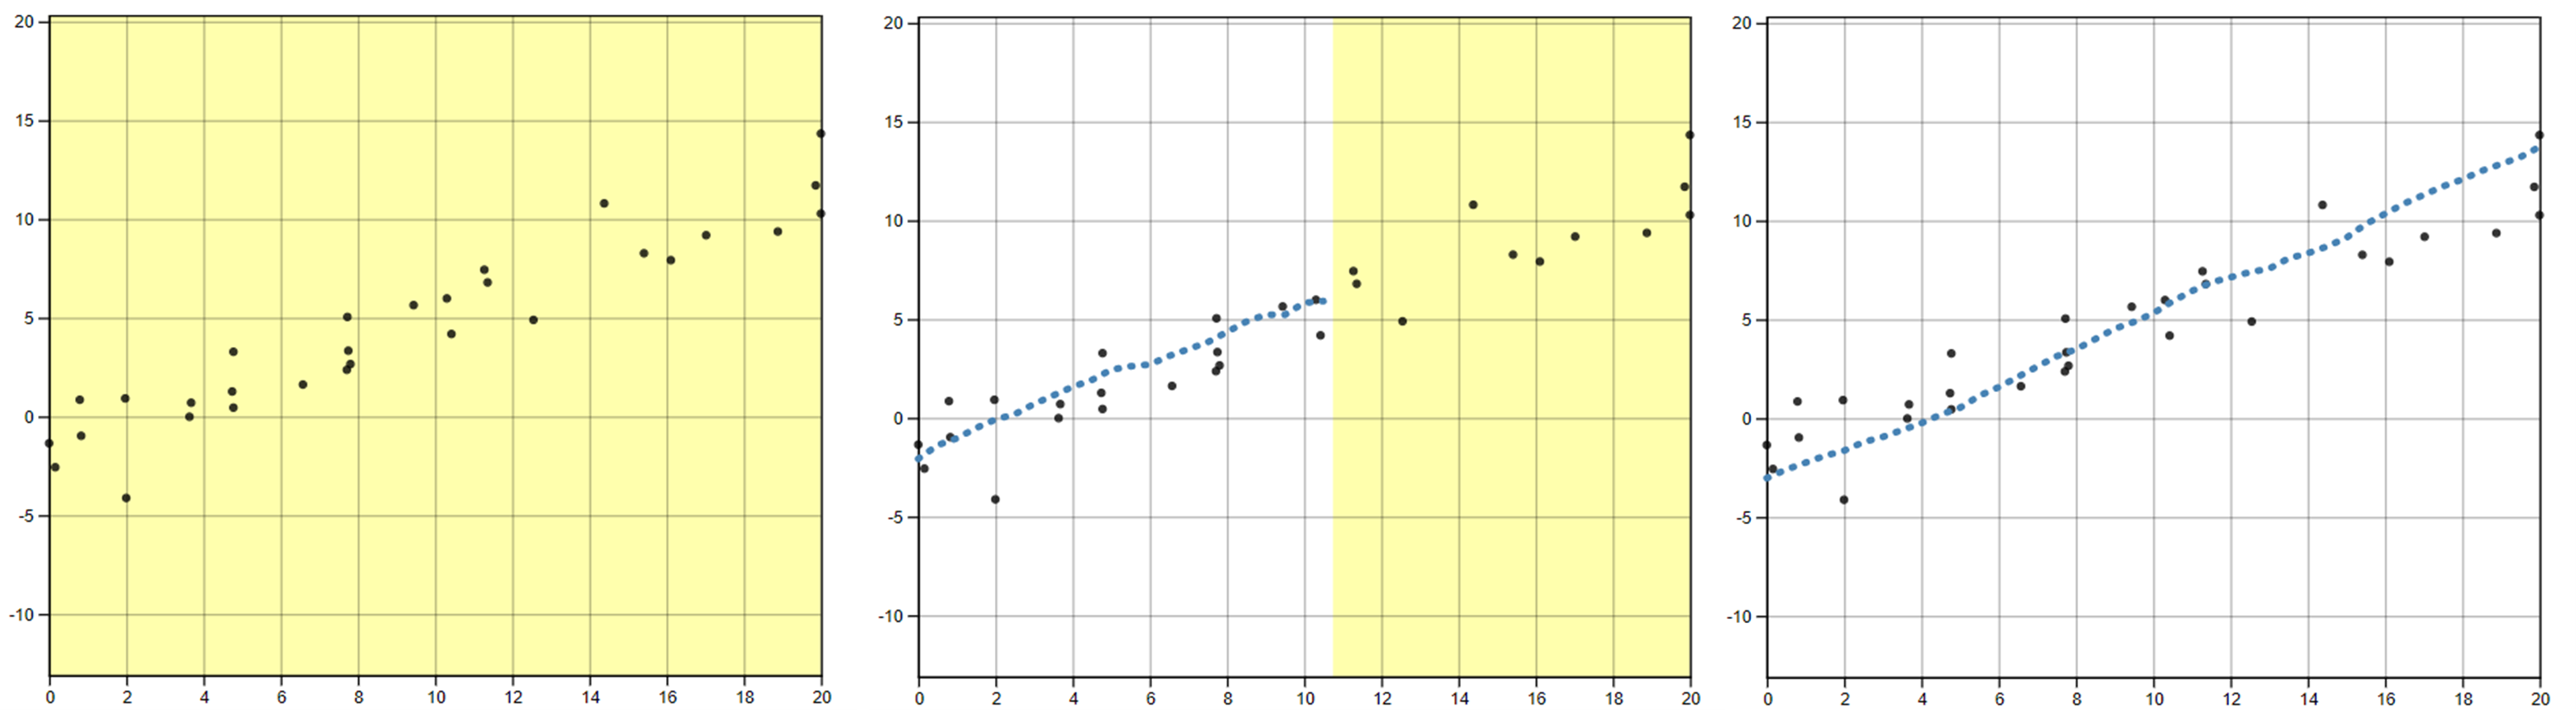
\includegraphics[width=1\linewidth,]{images/ydi-stimuli} 

}

\caption{'You Draw It' task plot as shown to particpants during the study. The first frame (left) illustrates what particpants first saw with the prompt “Use your mouse to fill in the trend in the yellow box region.” The second frame (middle), illustrates what the particpant saw while completing the task; the yellow shaded region provided a visual cue for participants indicating where the participant still needed to complete a trend-line. The last frame (right) illustrates the participants finished trend-line before submission.}\label{fig:ydi-stimuli}
\end{figure}

\hypertarget{data-generation}{%
\subsection{Data Generation}\label{data-generation}}

All data processing was conducted in R \DIFdelbegin \DIFdel{statistical software }\DIFdelend \DIFaddbegin \DIFadd{software environment for
statistical computing and graphics \mbox{%DIFAUXCMD
\citep{Rsoftware}}\hspace{0pt}%DIFAUXCMD
}\DIFaddend . A total of
\(N = 30\) points \DIFdelbegin \DIFdel{\((x_i, y_i), i = 1,...N\) }\DIFdelend \DIFaddbegin \DIFadd{\((x_i, y_i), i = 1,...,N\) }\DIFaddend were generated for
\(x_i \in [x_{min}, x_{max}]\) where \(x\) and \(y\) have a linear
relationship. Data were simulated based on \DIFaddbegin \DIFadd{the point-slope form of }\DIFaddend a
linear model with additive errors: \begin{align}
y_i \DIFdelbegin %DIFDELCMD < & %%%
\DIFdelend = \beta\DIFdelbegin \DIFdel{_0 + \beta}\DIFdelend _1\DIFaddbegin \DIFadd{(}\DIFaddend x_i\DIFaddbegin \DIFadd{-}\bar{x}\DIFadd{) + y_{\bar{x}} }\DIFaddend + e_i \\
\text{with } e_i & \sim N(0, \sigma^2). \nonumber
\end{align}

Model equation parameters, \DIFdelbegin \DIFdel{\(\beta_0\) and }\DIFdelend \(\beta_1\), \DIFaddbegin \DIFadd{\(y_{\bar{x}}\), and parameter
choice letter names (S, F, V, N), }\DIFaddend were selected to reflect the four data
sets \DIFdelbegin \DIFdel{(F, N, S, and V) used }\DIFdelend \DIFaddbegin \DIFadd{used and labeled }\DIFaddend in \citet{mosteller1981eye}
(\cref{tab:eyefitting-parameters}). \DIFdelbegin \DIFdel{We obtained
\(\beta_0\) from the point-slope equation of a line using the }\DIFdelend \DIFaddbegin \DIFadd{The }\DIFaddend mean of the generated \(x\)
values and the predefined \(y\) value at \(\bar x\), denoted
\(y_{\bar x}\) \DIFaddbegin \DIFadd{were used in the point-slope equation of a line}\DIFaddend .
Parameter choices \DIFdelbegin \DIFdel{F, N, and S }\DIFdelend \DIFaddbegin \DIFadd{S, F, and N }\DIFaddend simulated data across a domain of 0 to 20.
Parameter choice F produced a trend with a positive slope and a large
variance while N had a negative slope and a large variance. In
comparison, S showed a trend with a positive slope and a small variance
while V yielded a steep positive slope with a small variance over the
domain of 4 to 16. \cref{fig:eyefitting-simplot} illustrates an example
of simulated data for all four parameter choices intended to reflect the
trends in \citet{mosteller1981eye}. Aesthetic design choices were made
consistent across each of the interactive `You Draw It' task plots. The
y-axis range extended 10\% beyond (above and below) the range of the
simulated data points to allow for users to draw outside the simulated
data set range and avoid anchoring their lines to the corners of the
plot.

\begin{table}

\caption{\label{tab:eyefitting-parameters}Designated model equation parameters for simulated data.}
\centering
\begin{tabular}[t]{ccccc}
\toprule
Parameter Choice & $y_{\bar{x}}$ & $\beta_1$ & $\sigma$ \DIFaddbeginFL & \DIFaddFL{Domain}\DIFaddendFL \\
\midrule
S & 3.88 & 0.66 & 1.30 \DIFaddbeginFL & \DIFaddFL{(0,20)}\DIFaddendFL \\
F & 3.90 & 0.66 & 1.98 \DIFaddbeginFL & \DIFaddFL{(0,20)}\DIFaddendFL \\
V & 3.89 & 1.98 & 1.50 \DIFaddbeginFL & \DIFaddFL{(4,16)}\DIFaddendFL \\
N & 4.11 & -0.70 & 2.50 \DIFaddbeginFL & \DIFaddFL{(0,20)}\DIFaddendFL \\
\bottomrule
\end{tabular}
\end{table}

\begin{figure}[tbp]

{\centering 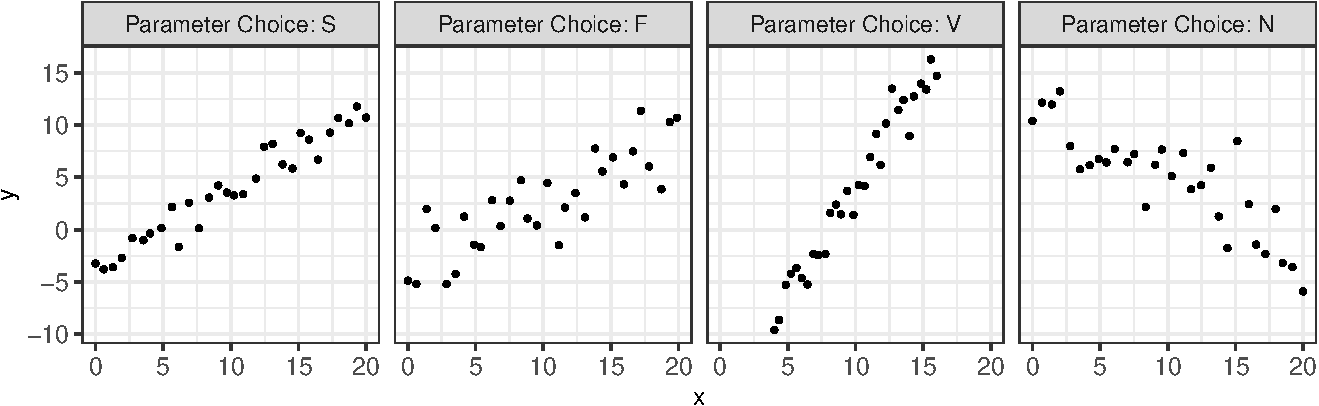
\includegraphics[width=1\linewidth,]{Eye-Fitting-Straight-Lines-in-the-Modern-Era_files/figure-latex/eyefitting-simplot-1} 

}

\caption{Example of simulated data points displayed in a \DIFdelbeginFL \DIFdelFL{scatter-plot }\DIFdelendFL \DIFaddbeginFL \DIFaddFL{scatterplot }\DIFaddendFL illustrating the trends associated with the four selected parameter choices.}\label{fig:eyefitting-simplot}
\end{figure}

\hypertarget{study-design}{%
\subsection{Study Design}\label{study-design}}

This experiment was conducted as part of a larger study of the
perception of log and linear scales; for simplicity, we focused on the
study design and methods related to the current study. Each \DIFdelbegin \DIFdel{scatter-plot
was the graphical representation of a data set that }\DIFdelend \DIFaddbegin \DIFadd{data set }\DIFaddend was
generated randomly and independently for each participant at the start
of the experiment \DIFaddbegin \DIFadd{and mapped to a scatterplot}\DIFaddend . Participants in the study
were shown two `You Draw It' practice plots in order to train
participants in the skills associated with executing the task - in
particular, the responsiveness of the applet requires that participants
draw a line at a certain speed, ensuring that all of the evenly spaced
points along the hand-drawn line are filled in. During the practice
session, participants were provided with instruction prompts accompanied
by a .gif and a practice plot. Instructions guided participants to start
at the edge of the yellow box, to make sure the yellow shaded region was
moving along with their mouse as they drew, and that they could draw
over their already drawn line. Practice plots were then followed by \DIFaddbegin \DIFadd{one
of each of the }\DIFaddend four `You Draw It' task plots associated with the current
study \DIFaddbegin \DIFadd{(S, F, V, and N)}\DIFaddend . The order of the task plots was randomly
assigned for each individual in a completely randomized design.

\hypertarget{results}{%
\section{Results}\label{results}}

\hypertarget{fitted-regression-lines}{%
\subsection{Fitted Regression Lines}\label{fitted-regression-lines}}

We compared the participant drawn line to two regression lines
determined by ordinary least squares (OLS) regression and regression
based on the principal axis (\DIFdelbegin \DIFdel{PCA}\DIFdelend \DIFaddbegin \DIFadd{PA}\DIFaddend ). \cref{fig:ols-vs-pca-example}
illustrates the difference between an OLS regression line which
minimizes the vertical distance of points from the line and a regression
line based on the \DIFdelbegin \DIFdel{principal axis }\DIFdelend \DIFaddbegin \DIFadd{PA }\DIFaddend which minimizes the Euclidean distance of points
(orthogonal) from the line.

Due to the randomness in the data generation process, the actual slope
of the linear regression line fit through the simulated points could
differ from the predetermined slope. Therefore, we fit an OLS regression
to each \DIFdelbegin \DIFdel{scatter-plot }\DIFdelend \DIFaddbegin \DIFadd{scatterplot }\DIFaddend to obtain estimated parameters \(\hat\beta_{0,OLS}\)
and \(\hat\beta_{1,OLS}\). Fitted values, \(\hat y_{k,OLS}\), were then
obtained every 0.25 \DIFdelbegin \DIFdel{increments }\DIFdelend \DIFaddbegin \DIFadd{increment }\DIFaddend across the domain from the OLS regression
equation,
\(\hat y_{k,OLS} = \hat\beta_{0,OLS} + \hat\beta_{1,OLS} x_k\)\DIFdelbegin \DIFdel{.}\DIFdelend , for
\(k = 1, ..., 4 x_{max} +1\). The \DIFdelbegin \DIFdel{regression equation based on the
principal axis was determined by using the }\DIFdelend \DIFaddbegin \DIFadd{PA regression slope,
\(\hat\beta_{1,PA}\), and y-intercept, \(\hat\beta_{0,PA}\), were
determined using the }\DIFaddend \texttt{\DIFdelbegin \DIFdel{princomp}\DIFdelend \DIFaddbegin \DIFadd{mcreg}\DIFaddend } function in the \DIFdelbegin \DIFdel{stats package
in base R to obtain the rotation of the coordinate
axes from the first principal component (direction which captures the most variance). The estimated slope , \(\hat\beta_{1,PCA}\), was
determined by the ratio of the axis rotation in \(y\) and axis rotation
in \(x\) }\DIFdelend \DIFaddbegin \texttt{\DIFadd{mcr}} \DIFadd{package
in R \mbox{%DIFAUXCMD
\citep{mcr_pkg} }\hspace{0pt}%DIFAUXCMD
which implements Deming regression (equivalent to a
regression based on the slope }\DIFaddend of the first principal \DIFdelbegin \DIFdel{component with the y-intercept,
\(\hat\beta_{0,PCA}\) calculated by the point-slope equation of a line
using the mean of the simulated points, \((\bar x_i, \bar y_i)\)}\DIFdelend \DIFaddbegin \DIFadd{axis)}\DIFaddend . Fitted
values, \DIFdelbegin \DIFdel{\(\hat y_{k,PCA}\), }\DIFdelend \DIFaddbegin \DIFadd{\(\hat y_{k,PA}\) }\DIFaddend were then obtained every 0.25 increment across
the domain from the \DIFdelbegin \DIFdel{PCA }\DIFdelend \DIFaddbegin \DIFadd{PA }\DIFaddend regression equation,
\DIFdelbegin \DIFdel{\(\hat y_{k,PCA} = \hat\beta_{0,PCA} + \hat\beta_{1,PCA} x_k\)}\DIFdelend \DIFaddbegin \DIFadd{\(\hat y_{k,PA} = \hat\beta_{0,PA} + \hat\beta_{1,PA} x_k\), for
\(k = 1, ..., 4 x_{max} +1\)}\DIFaddend .

\begin{figure}[tbp]

{\centering 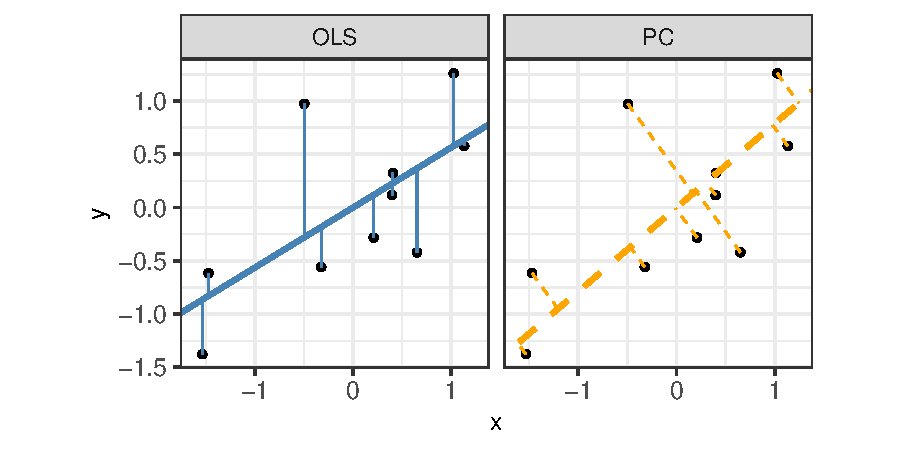
\includegraphics[width=0.8\linewidth,]{Eye-Fitting-Straight-Lines-in-the-Modern-Era_files/figure-latex/ols-vs-pca-example-1} 

}

\caption{ Comparison between an OLS regression line which minimizes the vertical distance of points from the line and a regression line based on the principal axis which minimizes the Euclidean distance of points (orthogonal) from the line.}\label{fig:ols-vs-pca-example}
\end{figure}

\hypertarget{residual-trends}{%
\subsection{Residual Trends}\label{residual-trends}}

For each participant, the final data set used for analysis contained
\(x_{ijk}, y_{ijk,drawn}, \hat y_{ijk,OLS}\), and \DIFdelbegin \DIFdel{\(\hat y_{ijk,PCA}\)
}\DIFdelend \DIFaddbegin \DIFadd{\(\hat y_{ijk,PA}\)
}\DIFaddend for parameter choice \(i = 1,2,3,4\), j = \DIFdelbegin \DIFdel{\(1,...N_{participant}\)}\DIFdelend \DIFaddbegin \DIFadd{\(1,...,N_{participant}\)}\DIFaddend , and
\(x_{ijk}\) value for increment \(k = 1, ...,4 x_{max} + 1\). Using both
a linear mixed model and a generalized additive mixed model, comparisons
of vertical residuals in relation to the OLS fitted values
(\(e_{ijk,OLS} = y_{ijk,drawn} - \hat y_{ijk,OLS}\)) and \DIFdelbegin \DIFdel{PCA }\DIFdelend \DIFaddbegin \DIFadd{PA }\DIFaddend fitted
values (\DIFdelbegin \DIFdel{\(e_{ijk,PCA} = y_{ijk,drawn} - \hat y_{ijk,PCA}\)}\DIFdelend \DIFaddbegin \DIFadd{\(e_{ijk,PA} = y_{ijk,drawn} - \hat y_{ijk,PA}\)}\DIFaddend ) were made
across the domain. \cref{fig:eyefitting-example-plot} displays an
example of all three fitted trend lines for parameter choice F.

\begin{figure}[tbp]

{\centering 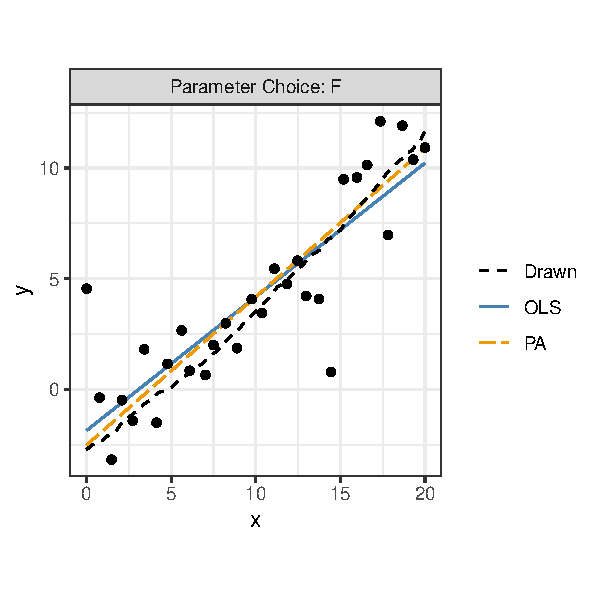
\includegraphics[width=0.5\linewidth,]{Eye-Fitting-Straight-Lines-in-the-Modern-Era_files/figure-latex/eyefitting-example-plot-1} 

}

\caption{Illustrates the data associated with and collected for one `You Draw It' task plot. Trend-lines include the participant drawn line (dashed black), the OLS regression line (solid steelblue) and the \DIFdelbeginFL \DIFdelFL{PCA }\DIFdelendFL \DIFaddbeginFL \DIFaddFL{PA }\DIFaddendFL regression line based on the principal axis (solid orange).}\label{fig:eyefitting-example-plot}
\end{figure}

\hypertarget{linear-trend-constraint}{%
\subsubsection{Linear Trend Constraint}\label{linear-trend-constraint}}

\DIFaddbegin \DIFadd{The `You Draw It' method does not restrict participants to draw a
straight line as other methods would, such as using a ruler. Instead,
participants are allowed to freely draw a line with potential curvature.
}\DIFaddend Using the \texttt{lmer} function in the lme4 package \citep{lme4}, a
linear mixed model (LMM) was fit separately to the OLS residuals and \DIFdelbegin \DIFdel{PCA
residuals, constraining the fit to }\DIFdelend \DIFaddbegin \DIFadd{PA
residuals, emulating the effect of constraining participants to draw }\DIFaddend a
linear trend. \DIFaddbegin \DIFadd{Both fixed and random parameter estimates in the LMM were
determined by optimizing the restricted maximum likelihood (REML)
through penalized least squares. }\DIFaddend Parameter choice, \(x\), and the
interaction between \(x\) and the parameter choice were treated as fixed
effects with a random participant effect included to account for
variation due to participant. The LMM equation for each fit (OLS and \DIFdelbegin \DIFdel{PCA}\DIFdelend \DIFaddbegin \DIFadd{PA}\DIFaddend )
is given by: \begin{equation}
y_{ijk,drawn} - \hat y_{ijk,fit} = e_{ijk,fit} = \left[\gamma_0 + \alpha_i\right] + \left[\gamma_{1} x_{ijk} + \gamma_{2i} x_{ijk}\right] + p_{j} + \epsilon_{ijk}
\end{equation} \noindent where

\begin{itemize}
\tightlist
\item
  \(y_{ijk,drawn}\) is the drawn \(y\) value for the \(i^{th}\)
  parameter choice, \(j^{th}\) participant, and \(k^{th}\) increment of
  \(x\) value
\item
  \(\hat y_{ijk,fit}\) is the fitted \(y\) value for the \(i^{th}\)
  parameter choice, \(j^{th}\) participant, and \(k^{th}\) increment of
  \(x\) value corresponding to either the OLS or \DIFdelbegin \DIFdel{PCA }\DIFdelend \DIFaddbegin \DIFadd{PA }\DIFaddend fit
\item
  \(e_{ijk,fit}\) is the residual between the drawn and fitted \(y\)
  values for the \(i^{th}\) parameter choice, \(j^{th}\) participant,
  and \(k^{th}\) increment of \(x\) value corresponding to either the
  OLS or \DIFdelbegin \DIFdel{PCA }\DIFdelend \DIFaddbegin \DIFadd{PA }\DIFaddend fit
\item
  \(\gamma_0\) is the overall intercept
\item
  \(\alpha_i\) is the effect of the \(i^{th}\) parameter choice (\DIFdelbegin \DIFdel{F, S, }\DIFdelend \DIFaddbegin \DIFadd{S, F,
  }\DIFaddend V, N) on the intercept
\item
  \(\gamma_1\) is the overall slope for \(x\)
\item
  \(\gamma_{2i}\) is the effect of the parameter choice on the slope
\item
  \(x_{ijk}\) is the \(x\) value for the \(i^{th}\) parameter choice,
  \(j^{th}\) participant, and \(k^{th}\) increment
\item
  \(p_{j} \sim N(0, \sigma^2_{participant})\) is the random error due to
  the \(j^{th}\) participant's characteristics
\item
  \(\epsilon_{ijk} \sim N(0, \sigma^2)\) is the residual error.
\end{itemize}

Constraining the residual trend to a linear fit,
\cref{fig:eyefitting-lmer-residualplots} shows the estimated trend line
of the residuals between the participant drawn points and fitted values
for both the OLS regression line and \DIFdelbegin \DIFdel{PCA }\DIFdelend \DIFaddbegin \DIFadd{PA }\DIFaddend regression line. Estimated
residual trend lines are overlaid on the observed individual participant
residuals. Results indicate the estimated trends of \DIFdelbegin \DIFdel{PCA }\DIFdelend \DIFaddbegin \DIFadd{PA }\DIFaddend residuals
(orange) appear to align closer to the \(y=0\) horizontal (dashed) line
than the OLS residuals (blue). In particular, this trend is more
prominent in parameter choices with large variances (F and N). These
results are consistent to those found in \citet{mosteller1981eye}
indicating participants fit a trend-line closer to the estimated
regression line with a slope based on the first principal axis than the
estimated OLS regression line\DIFdelbegin \DIFdel{thus, providing support for ``ensemble
perception''}\DIFdelend .

\begin{figure}[tbp]

{\centering 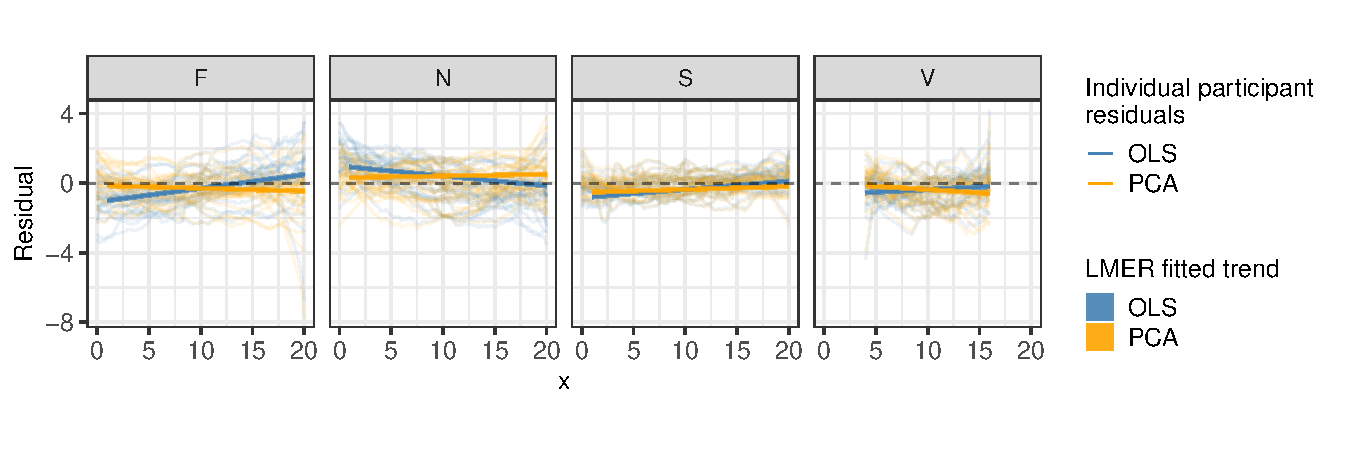
\includegraphics[width=1\linewidth,]{Eye-Fitting-Straight-Lines-in-the-Modern-Era_files/figure-latex/eyefitting-lmer-residualplots-1} 

}

\caption{Estimated trend line of the residuals between the participant drawn points and fitted values for both the OLS (blue) regression line and \DIFdelbeginFL \DIFdelFL{PCA }\DIFdelendFL \DIFaddbeginFL \DIFaddFL{PA }\DIFaddendFL (orange) regression line constrained to a linear fit modeled by a linear mixed model. Estimated residual trends with 95\% confidence bands are overlaid on the observed individual participant residuals.}\label{fig:eyefitting-lmer-residualplots}
\end{figure}

\hypertarget{smoothing-spline-trend}{%
\subsubsection{Smoothing Spline Trend}\label{smoothing-spline-trend}}

Eliminating the linear trend constraint, the \texttt{bam} function in
the mgcv package \DIFdelbegin \DIFdel{\mbox{%DIFAUXCMD
\citep{mgcv1, mgcv2, mgcv3, mgcv4, mgcv5} }\hspace{0pt}%DIFAUXCMD
}\DIFdelend \DIFaddbegin \DIFadd{\mbox{%DIFAUXCMD
\citep{mgcv_pkg} }\hspace{0pt}%DIFAUXCMD
}\DIFaddend was used to fit a generalized additive
mixed model (GAMM) separately to the OLS residuals and \DIFdelbegin \DIFdel{PCA }\DIFdelend \DIFaddbegin \DIFadd{PA }\DIFaddend residuals to
allow for estimation of smoothing splines. \DIFaddbegin \DIFadd{The }\texttt{\DIFadd{bam}} \DIFadd{function is
used to fit GAMM's to very large data sets and use lower memory than the
}\texttt{\DIFadd{gam}} \DIFadd{function; REML is used to estimate parameters and smoothing
splines. }\DIFaddend Parameter choice was treated as a fixed effect with no
estimated intercept and a separate smoothing spline for \(x\) was
estimated for each parameter choice. A random participant effect was
included to account for variation due to participant and a random spline
for each participant accounted for variation in spline for each
participant. \DIFdelbegin \DIFdel{The }\DIFdelend \DIFaddbegin \DIFadd{Defining e\_\{ijk,fit\} the same as in equation (2) above,
the }\DIFaddend GAMM equation for each fit (OLS and \DIFdelbegin \DIFdel{PCA}\DIFdelend \DIFaddbegin \DIFadd{PA}\DIFaddend ) residuals is given by:
\begin{equation}
\DIFdelbegin \DIFdel{y_{ijk, drawn} - }%DIFDELCMD < \hat %%%
\DIFdel{y_{ijk, fit} = }\DIFdelend e_{ijk,fit} = \alpha_i + s_{i}(x_{ijk}) + p_{j} + s_{j}(x_{ijk})
\end{equation} \noindent where

\begin{itemize}
\tightlist
\item
  \DIFdelbegin \DIFdel{\(y_{ijk,drawn}\) is the drawn \(y\) value for the \(i^{th}\)
  parameter choice, \(j^{th}\) participant, and \(k^{th}\) increment of
  \(x\) value
}%DIFDELCMD < \item
\item%DIFAUXCMD
%DIFDELCMD <   %%%
\DIFdel{\(\hat y_{ijk,fit}\) is the fitted \(y\) value for the \(i^{th}\)
  parameter choice, \(j^{th}\) participant, and \(k^{th}\) increment of
  \(x\) value corresponding to either the OLS or PCA fit
}%DIFDELCMD < \item
\item%DIFAUXCMD
%DIFDELCMD <   %%%
\DIFdelend \(e_{ijk,fit}\) is the \DIFdelbegin \DIFdel{residual between the drawn and fitted \(y\)
  values for the \(i^{th}\) parameter choice, \(j^{th}\) participant,
  and \(k^{th}\) increment of \(x\) value corresponding to either the
  OLS or PCA fit
}\DIFdelend \DIFaddbegin \DIFadd{same as equation
}\DIFaddend \item
  \(\alpha_i\) is the intercept for the parameter choice \(i\)
\item
  \(s_{i}\) is the smoothing spline for the \(i^{th}\) parameter choice
\item
  \(x_{ijk}\) is the \(x\) value for the \(i^{th}\) parameter choice,
  \(j^{th}\) participant, and \(k^{th}\) increment
\item
  \(p_{j} \sim N(0, \sigma^2_{participant})\) is the error due to
  participant variation
\item
  \(s_{j}\) is the random smoothing spline for each participant.
\end{itemize}

Allowing for flexibility in the residual trend,
\cref{fig:eyefitting-gamm-residualplots} shows the estimated trend line
of the residuals between the participant drawn points and fitted values
for both the OLS regression line and \DIFdelbegin \DIFdel{PCA }\DIFdelend \DIFaddbegin \DIFadd{PA }\DIFaddend regression line. Estimated
residual trends were overlaid on the observed individual participant
residuals. The results of the GAMM align with those shown in
\cref{fig:eyefitting-lmer-residualplots} providing support that
estimated trends of \DIFdelbegin \DIFdel{PCA }\DIFdelend \DIFaddbegin \DIFadd{PA }\DIFaddend residuals (orange) appear to align closer to the
\(y=0\) horizontal (dashed) line than the OLS residuals (blue) for
\DIFdelbegin \DIFdel{scatter-plots }\DIFdelend \DIFaddbegin \DIFadd{scatterplots }\DIFaddend with more noise (F and N). By fitting smoothing splines, we
can determine whether participants naturally fit a straight trend-line
to the set of points or whether they deviate throughout the domain. In
particular, in \DIFdelbegin \DIFdel{scatter-plots }\DIFdelend \DIFaddbegin \DIFadd{scatterplots }\DIFaddend with smaller variance (S and V), we can see
that participants began at approximately the correct starting point then
deviated away from the fitted regression lines and corrected for their
fit toward the end of their trend-line. In \DIFdelbegin \DIFdel{scatter-plots }\DIFdelend \DIFaddbegin \DIFadd{scatterplots }\DIFaddend with larger
variance (F and N), participants estimated their starting value in the
extreme direction of the OLS regression line based on the increasing or
decreasing trend but more accurately represented the starting value of
the \DIFdelbegin \DIFdel{PCA }\DIFdelend \DIFaddbegin \DIFadd{PA }\DIFaddend regression line. As participants continued their trend-line, they
crossed through the OLS regression line indicating they estimated the
slope in the extreme direction. These results provide further insight
into the curvature humans perceive in a set of points.

\begin{figure}[tbp]

{\centering 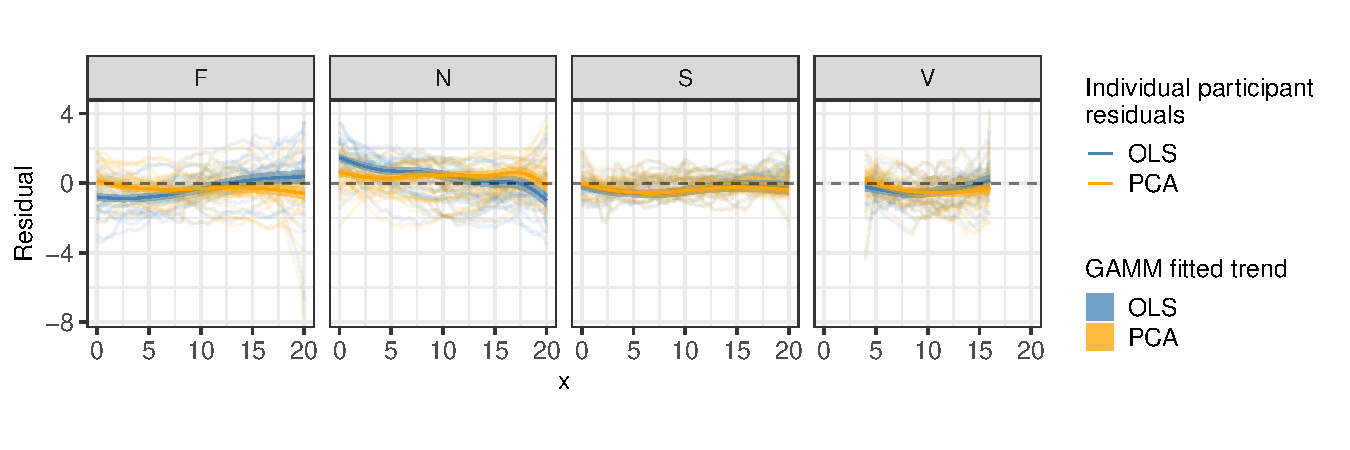
\includegraphics[width=1\linewidth,]{Eye-Fitting-Straight-Lines-in-the-Modern-Era_files/figure-latex/eyefitting-gamm-residualplots-1} 

}

\caption{Estimated trend line of the residuals between the participant drawn points and fitted values for both the OLS (blue) regression line and \DIFdelbeginFL \DIFdelFL{PCA }\DIFdelendFL \DIFaddbeginFL \DIFaddFL{PA }\DIFaddendFL (orange) regression line determined by smoothing splines fit by a generalized additive mixed model. Estimated residual trends with 95\% confidence bands are overlaid on the observed individual participant residuals.}\label{fig:eyefitting-gamm-residualplots}
\end{figure}

\DIFdelbegin %DIFDELCMD < \hypertarget{discussion-and-conclusion}{%
%DIFDELCMD < \section{Discussion and Conclusion}\label{discussion-and-conclusion}}
%DIFDELCMD < %%%
\DIFdelend \DIFaddbegin \hypertarget{conclusion-discussion}{%
\section{Discussion and Conclusion}\label{conclusion-discussion}}
\DIFaddend 

The intent of this research was to adapt `You Draw It' from the New York
Times feature as a tool and method for testing graphics and introduce a
method for statistically modeling the participant drawn lines. We
provided support for the validity of the `You Draw It' method by
replicating the study found in \citet{mosteller1981eye}. Using
generalized additive mixed models, we assessed the deviation of the
participant drawn lines from the statistically fitted regression lines.
Our results found that when shown points following a linear trend,
participants visually fit a regression line that mimics the first
\DIFdelbegin \DIFdel{principle component }\DIFdelend \DIFaddbegin \DIFadd{principal axis }\DIFaddend regression as opposed to ordinary least squares
regression. Data simulated with a larger variance provided strong
support for a participants tendency to visually fit the first \DIFdelbegin \DIFdel{principle
component }\DIFdelend \DIFaddbegin \DIFadd{principal
axis }\DIFaddend regression. We utilized modern technology to replicate a study
conducted 40 years ago, and strengthened the original results with
current analysis methods which allow for more flexibility and
sophistication. Our results indicate that participants minimized the
distance from their drawn regression line over both the \(x\) and \(y\)
axis simultaneously. \DIFdelbegin \DIFdel{These results provide support that humans perform
``ensemble perception'' in a statistical graphic setting. }\DIFdelend We allowed participants to draw trend lines that
deviated from a straight line and gained an insight into the curvature
the human eye perceives in a set of points. \DIFaddbegin \DIFadd{Researchers in cognitive and
human movement sciences have found that human arm movement is a complex
task \mbox{%DIFAUXCMD
\citep{miall1995curvature, rousset2015study}}\hspace{0pt}%DIFAUXCMD
. The `You Draw It'
method described in this paper uses }\emph{\DIFadd{indirect interaction}} \DIFadd{in which
the mouse position and resulting visual line on the screen are
dissociated. Therefore, curvature found in participant drawn lines from
a straight lines could potentially be explained by the lack of
coordination which results from the eye-hand dissociation from indirect
drawing and the distortion of visual perception affecting the curvature
of movements. Additionally, there is a training effect related to the
completion of the `You Draw It' task - the movement of the line must be
slow so that the visual representation on the screen can accurately
capture each movement. \mbox{%DIFAUXCMD
\citet{de1991misdirections} }\hspace{0pt}%DIFAUXCMD
conducted a study in
which participants moved their hand slowly from an initial position in
front of them to a visual target (movement task); they were then asked
to repeat the task using different sizes of pointers (perceptual task).
Their results indicated that deviations from the shortest pointers were
comparable to those of the movement task, but that bias increased as the
length of the pointer increased. While we suggested participants use a
mouse to complete the study, we could not require the use; therefore,
some participants may have used a track-pad and results may have been
influenced by the pressure placed on their track-pad
\mbox{%DIFAUXCMD
\citep{easton1978finger}}\hspace{0pt}%DIFAUXCMD
.
}\DIFaddend 

\hypertarget{future-work}{%
\section{Future Work}\label{future-work}}

This study provided a basis for the use of `You Draw It' as a tool for
testing statistical graphics and introduced a method for statistically
modeling participant drawn lines using generalized additive mixed
models. \DIFdelbegin \DIFdel{Further }\DIFdelend \DIFaddbegin \DIFadd{Additional studies related to the validation and use of the tool
would be useful for providing insight into explanations of biases
introduced by the task such as the deviation from a straight line. For
instance, a variation on the current study could compare manual
adjustment methods such as shifting and rotating a horizontal line
segment until the fit is suitable to the `You Draw It' method on the
same set of data. This might explain the large deviation from the
participant drawn line as \(x\) approaches 20. Another useful extension
study would be to compare the `You Draw It' method as conducted by
direct interaction - using a digital pen on a tablet - to indirect
interaction - using a computer mouse to relate to a pointer on the
screen. Further extensions to this work might ask participants to draw a
trend-line through scatterplots with one (or multiple) extreme outliers
in order to evaluate the perceptual system's resistance to outliers.
}

\DIFadd{While the focus of this study was on drawing linear trend-lines, further
}\DIFaddend investigation is necessary to implement this method in non-linear
settings and with real data in order to facilitate scientific
communication \DIFaddbegin \DIFadd{- a strength of the combination of the flexible `You Draw
It' method and GAMM analysis method}\DIFaddend . This tool could also be used to
evaluate human ability to extrapolate data from trends. In the future,
we intend to create an R package designed for easy implementation of
`You Draw It' task plots in order to make this tool accessible to other
researchers.

\DIFdelbegin %DIFDELCMD < \begin{center}
%DIFDELCMD < {\large\bf %%%
\DIFdel{SUPPLEMENTARY MATERIAL}%DIFDELCMD < }
%DIFDELCMD < \end{center}
%DIFDELCMD < %%%
\DIFdelend \DIFaddbegin \hypertarget{supplementary-material}{%
\section{SUPPLEMENTARY MATERIAL}\label{supplementary-material}}
\DIFaddend 

\begin{itemize}
\tightlist
\item
  \DIFaddbegin \textbf{\DIFadd{Study Applet:}} \DIFadd{The shiny app used to conduct the study can be
  accessed at
  }\href{https://emily-robinson.shinyapps.io/you-draw-it-validation-applet/}{emily-robinson.shinyapps.io/you-draw-it-validation-applet}\DIFadd{.
}\item
  \textbf{\DIFadd{RShiny Applet Code:}} \DIFadd{The code used to create the RShiny Applet
  for data collection can be found at
  }\href{https://github.com/earobinson95/you-draw-it-validation-applet}{github.com/earobinson95/you-draw-it-validation-applet}\DIFadd{.
}\item
  \DIFaddend \textbf{Participant Data:} De-identified participant data collected in
  the study and used for analyses are available to be downloaded from
  GitHub \DIFdelbegin %DIFDELCMD < \href{https://github.com/earobinson95/Eye-Fitting-Straight-Lines-in-the-Modern-Era/tree/main/data}{here}%%%
\DIFdelend \DIFaddbegin \DIFadd{at
  }\href{https://github.com/earobinson95/Eye-Fitting-Straight-Lines-in-the-Modern-Era/tree/main/data}{github.com/earobinson95/Eye-Fitting-Straight-Lines-in-the-Modern-Era/tree/main/data}\DIFaddend .
\item
  \textbf{Data Analysis Code:} The code used to replicate the analysis
  in this paper can be found \DIFdelbegin %DIFDELCMD < \href{https://earobinson95.github.io/Eye-Fitting-Straight-Lines-in-the-Modern-Era/analysis/you-draw-it-eyefitting-analysis.html}{here}%%%
\DIFdel{.
}%DIFDELCMD < \item
\item%DIFAUXCMD
%DIFDELCMD <   %%%
\textbf{\DIFdel{Study Applet:}} %DIFAUXCMD
\DIFdel{The shiny app used to conduct the study can be
  accessed
  }%DIFDELCMD < \href{https://emily-robinson.shinyapps.io/you-draw-it-validation-applet/}{here}%%%
\DIFdel{.
}%DIFDELCMD < \item
\item%DIFAUXCMD
%DIFDELCMD <   %%%
\textbf{\DIFdel{RShiny Applet Code:}} %DIFAUXCMD
\DIFdel{The code used to create the RShiny Applet
  for data collection can be found
  }%DIFDELCMD < \href{https://github.com/earobinson95/you-draw-it-validation-applet}{here}%%%
\DIFdelend \DIFaddbegin \DIFadd{at
  }\href{https://earobinson95.github.io/Eye-Fitting-Straight-Lines-in-the-Modern-Era/analysis/you-draw-it-eyefitting-analysis.html}{earobinson95.github.io/Eye-Fitting-Straight-Lines-in-the-Modern-Era/analysis/you-draw-it-eyefitting-analysis.html}\DIFaddend .
\end{itemize}

\bibliographystyle{agsm}
\bibliography{bibliography.bib}


\end{document}
